\documentclass[titlepage]{article}
\usepackage[utf8]{inputenc}
\usepackage[margin=1.0in]{geometry}

\title{Balloon Catheter Training Device User Manual}
\author{Nam Tran\\ Biomedical Engineering\thanks{Undergraduate}, The George Washington University}
\date{November 2018}

\usepackage[english]{babel}
\usepackage{graphicx}

\begin{document}

\maketitle

\section{Introduction}
Balloon catheterization in this case is used for transvenous cardiac pacing, often utilised in the emergency department. This user manual describes a step-by-step narrative for using the device, referencing the objectives, functions, and user stories specified in this section. All user stories, objectives, and functions can be found in "Backgrounds, Vision, and Needs" \cite{backgroundreport}.

\subsection{User Stories}
The following user stories were derived from the needs presented by our client, Dr. Claudia Ranniger.

\begin{enumerate}
  \item The labels consists of sequential numbers.
  \item The numbers starts at 1 with every call to the enumerate environment.
\end{enumerate}


\subsection{Objectives}
The following objectives were considered in the engineering design of the device.

\begin{enumerate}
  \item The labels consists of sequential numbers.
  \item The numbers starts at 1 with every call to the enumerate environment.
\end{enumerate}


\subsection{Functions}
The following functions were required to meet our objectives.

\begin{enumerate}
  \item The labels consists of sequential numbers.
  \item The numbers starts at 1 with every call to the enumerate environment.
\end{enumerate}


\section{Narrative}

\begin{figure}[h!]
\centering
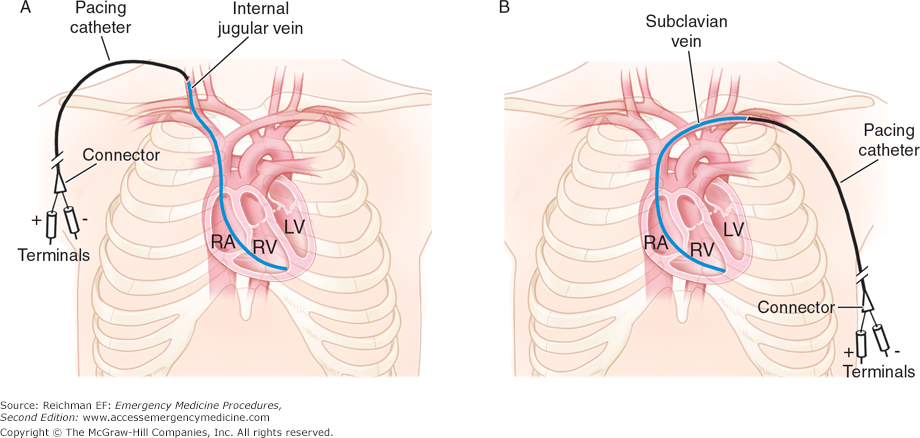
\includegraphics[scale=0.5]{transvenous}
\caption{Catheter path through the jugular vein and subclavian vein \cite{reichman2013emprocedures}}
\label{fig:universe}
\end{figure}

\clearpage
\bibliographystyle{ieeetr}
\bibliography{references}
\end{document}
